\newpage
\visHeader

\begin{figure}[htbp]
    \centering
    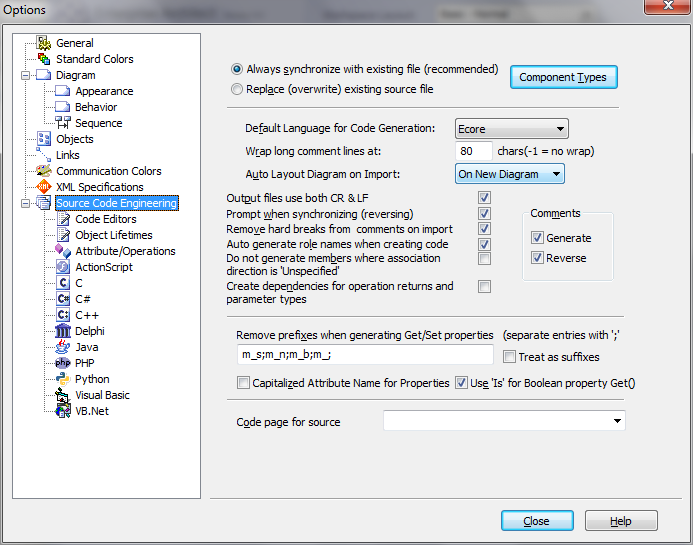
\includegraphics[width=0.8\textwidth]{standardCodeEngineering}
    \caption{Make sure you set the standard language to Ecore.}
    \label{fig_standardSCEEA}
 \end{figure}

with a certain project structure according to our conventions.  
The  \texttt{model} subfolder is probably most important, and contains an  \emph{Ecore model}.  
Ecore is a metamodelling language that provides building  blocks like \emph{classes} and \emph{references} for defining the  static structure (concepts and relations between concepts) of a system.  



The  export function of our EA plugin generates a valid Ecore model from the  corresponding EA model and persists it as an XML file in the \texttt{model}  subfolder.  
In our concrete example, this is the \texttt{DoubleLinkedListLanguage.ecore} file.  
Go ahead and double-click it to open the file in a simple tree-view editor in Eclipse.  
If you are really interested in the nitty-gritty details or have a masochistic hang, right-click the file and select ``Open With/Text Editor''.


This Ecore model is used to drive a code generator that maps the model to Java interfaces and classes.  
The generated Java code that represents the model is often referred to as a \emph{repository} and this is the reason why we refer to such projects as repository projects\footnote{Not to be mixed up with CVS or SVN repositories, although the idea of a source code ``container'' is the same here.}. 
A repository can be viewed as an \emph{adapter} that enables building and manipulating concrete instances of a specific model via a programming language such as Java.  
This is why we indicate repository projects using a cute adapter/plug symbol on the project folder.  